\documentclass{article}
\usepackage{graphicx} % Required for inserting images
\usepackage{graphicx} % Required for inserting images
\usepackage{listings}
\usepackage{xcolor}
\usepackage{hyperref}

\newcommand\subsubsection{\@startsection{subsubsection}{3}{\z@}%
                {-3.25ex\@plus -1ex \@minus -.2ex}%
                {1.5ex \@plus .2ex}%
                {\normalfont\normalsize\bfseries}}


\definecolor{codegreen}{rgb}{0,0.6,0}
\definecolor{codegray}{rgb}{0.5,0.5,0.5}
\definecolor{codepurple}{rgb}{0.58,0,0.82}
\definecolor{backcolour}{rgb}{0.95,0.95,0.92}

\lstdefinestyle{mystyle}{
    backgroundcolor=\color{backcolour},   
    commentstyle=\color{codegreen},
    keywordstyle=\color{magenta},
    numberstyle=\tiny\color{codegray},
    stringstyle=\color{codepurple},
    basicstyle=\ttfamily\footnotesize,
    breakatwhitespace=false,         
    breaklines=true,                 
    captionpos=b,                    
    keepspaces=true,                 
    numbers=left,                    
    numbersep=5pt,                  
    showspaces=false,                
    showstringspaces=false,
    showtabs=false,                  
    tabsize=2
}

\lstset{style=mystyle}

\title{Compulsory assignment 2}
\author{Lars Haukland }
\date{October 2023}

\begin{document}


\section{Exercise 1}
\subsection{Simplify the following, using $\Theta$-notation}
Simplifying with big theta is similar to simplifying with big O, the difference is just that with big theta it is the best case for big O. Therefore since we know the whole expression it is easy to see big theta as we just focus on the largest part of the expression.
\begin{enumerate}
    \item $3n^3 + 2n - 4n^2$ can be simplified into $\Theta(n^3)$
    \item $13n^2 + n/n^2$ can be simplified into $\Theta(n^2)$
    \item $n^2 + n \log_3n$ can be simplified into $\Theta(n^2)$
\end{enumerate}

\subsection{Use the master theorem to find the following in O-notation}
The masters theorem is as follows.\\
For a function $T(n) \leq a\ T(\frac{n}{b}) + O(n^d)$ it follows that\\
If $d > log_b\ a => O(n^d)$ (Case 1)\\
If $d = log_b\ a => O(n^d\ log n)$ (Case 2)\\
If $d < log_b\ a => O(n^{log_b\ a}$ (Case 3)\\ \\
To solve the following recurrence relations I will write out the relation and then the big O for that recurrence relation. After this, the case that resulted in that big O will follow and the variables a, b and d. For example \\
$T(n) = 2T(\frac{n}{2}) + n = O(n\ log\ n)$, (Case 2), $a = 2, b = 2, d = 1$
\begin{enumerate}
    \item $T(n) = 4T(\frac{n}{2}) + n = O(n^2)$, (Case 3), $a = 4, b = 2, d = 1$
    \item $T(n) = 4T(\frac{n}{2}) + n\sqrt{n} = O(n^2)$, (Case 3), $a = 4, b = 2, d = \frac{3}{2}$
    \item $T(n) = 4T(\frac{n}{2}) + n^2 = O(n^2\ log\ n)$, (Case 2), $a = 4, b = 2, d = 2$
    \item $T(n) = 5T(\frac{n}{2}) + n = O(n^{log_2\ 5}) = O(n^{3.22})$ (Case 3), $a = 5, b = 2, d = 1$
    \item $T(n) = 5T(\frac{n}{2}) + n\sqrt{n} = O(n^{log_2\ 5} = O(n^{3.22})$ (Case 3), $a = 5, b = 2, d = \frac{3}{2}$
    \item $T(n) = 5T(\frac{n}{2}) + n^2 = O(n^{log_2\ 5}) = O(n^{3.22})$ (Case 3), $a = 5, b = 2, d = 2$
    \item $T(n) = 10T(\frac{n}{3}) + O(n\sqrt{n}) + 13 = O(n^{log_3\ 10}) = O(n^{2.096})$ (Case 3), $a = 10, b = 3, d = \frac{3}{2}$
\end{enumerate}

\subsection{Prove by induction that $T (n) = 2T (\frac{n}{2}) + cn$ is $O(n\ log\ n)$.}
\subsubsection{Base case, n=2}
From the formula to prove we can define that $T(n) \leq c\ n\ log\ n$\\
This we can substitute in the original formula to end up with\\
$T(n) = 2(c * \frac{n}{2} * log\frac{n}{2}) + c\ n$\\ \\
With n=2 we get: \\
$T(2) = 2(c * \frac{2}{2} * log\frac{2}{2}) + c\ n$\\
Here because both fractions end up being 2/2 and the logarithm of 1 is 0 this whole $2(c * \frac{2}{2} * log\frac{2}{2})$ ends up being 0 and we end up with: \\
$T(2) = 2\ c$ \\
This holds up because:
$T(2) = 2 \ c \leq c\ n\ log\ n$ (n=2) \\
$2\ c \leq 2\ c * log\ 2 => 2\ c \leq 2\ c$

\subsubsection{Induction hypothesis}
$\forall_{m>2}\ T(m) \leq c\ m\ log\ m$

\subsubsection{Inductive step (proving our hypothesis)}
$T(m) = 2T(\frac{m}{2}) + c\ n\\\\
= 2(c\ \frac{m}{2}\ log\frac{m}{2}) + c\ n \\\\
= c\ m\ log\frac{m}{2} + c\ m \\\\
= c\ m\ (log\ m - log\ 2 + 1)$ And this needs to be less than $c\ m\ log\ m$ for our proof to hold\\\\
$= c\ m\ (log\ m - log\ 2 + 1) \leq c\ m\ log\ m \\ \\
=> c\ m\ log\ m \leq c\ m\ log\ m$\\\\
This holds and proves that $T (n) = 2T (\frac{n}{2}) + cn$ is $O(n\ log\ n)$

\section{Exercise 2}
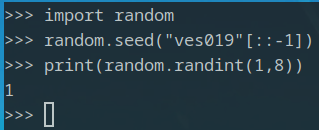
\includegraphics[scale=0.5]
{task-random.png}

\section{Exercise 3}
Implement the simplest possible algorithm in Python for exactly one of the
following, namely the one corresponding to the answer of Exercise 2. The
algorithm should use the time complexity we saw in class. Explain what the
complexity is, and give a short explanation for why it is correct.\\\\
As in the first compulsory exercise, we value elegance and simplicity over en-
gineering. Write the shortest possible readable code that solves the problem
correctly in the running time we have discussed in class.\\\\
For the main function you are implementing, give the docstring stating explicitly
the expected input and output.\\\\

\subsection{Counting Inversions}
The input here is two lists A and B and it should count how many inversions
there are in B given the items in A as “ground truth”. Note that you can simply
“relabel” the items in B according to their indices in A, and then run the one-list
version.\\
\begin{lstlisting}[language=Python]
def count_inversions(A, B):
    pass
\end{lstlisting}
The following algorithm is really just mergesort with some extra linear time steps. First there is pre-processing of the list B as the typical mergesort only handles one list we need to relabel all items in B based on A. Then comes the algorithm, that is very equal to mergesort. And we are actually sorting the list as in mergesort, the only difference is that we count everytime we "invert" two elements. An example is the list [2,1] to sort this we need to "invert" these two elements so that it ends up as [1,2]. 
\\ \\
Finally the algorithm returns a tuple with (number of inversions, new sorted list)
\lstinputlisting[language=Python]
{countingInversions.py}

\section{Exercise 4}

\paragraph{When is a problem in P?}
A problem is in the complexity class P when there exists an algorithm that can solve it in polynomial time worst case. This means that there exists an algorithm for the problem with time complexity $O(nk)$ where k is an integer.

\paragraph{When is a problem in NP?}
Wikipedia states it as: "NP is the set of problems that can be solved in polynomial time by a non deterministic Turing machine." (NP (complexity) 2023) This means that a problem is in NP if it can be solved in polynomial time by a non deterministic Turing machine. We can also say that a problem is NP if a solution can be guessed and verified in polynomial time.

\paragraph{How do we show that a problem is NP-complete?}
Here Britannica explains it nicely: "If a problem is NP and all other NP problems are polynomial-time reducible to it, the problem is NP-complete." (NP-complete problem 2023). An example of a NP-complete problem is Set Cover, we have other NP problems such as Vertex Cover that can be reduced to Set Cover.


\section{Sources}
\begin{enumerate}
    \item NP-complete problem (2023) Encyclopædia Britannica. Available at: \url{https://www.britannica.com/science/NP-complete-problem} (Accessed: 08 November 2023). 
    \item NP (complexity) (2023) Wikipedia. Available at: \url{https://en.wikipedia.org/wiki/NP_(complexity)} (Accessed: 08 November 2023).
\end{enumerate}

\end{document}
